\section{Numeryczny regulator predykcyjny MPCS}
\indent W numerycznym regulatorze w każdej chwili $k$ rozwiązywane jest zadanie programowania kwadratowego, które uwzględnia ograniczenia sterowania. Znacznie zwiększa to już i tak dosyć długi czas obliczeń, dlatego przedstawione zostały jedynie przypadki tych regulatorów dla niewielkich wartości horyzontów, przez co jakość regulacji jest względnie niska. Musi również istnieć rozwiązanie quadprog dla danych trajektorii wartości zadanych, zostały więc one zmienione, żeby sterowanie było nieco prostsze. \\ \indent Wykresy przedstawiają działanie regulatora analitycznego oraz numerycznego dla takich samych parametrów regulatora. Regulator numeryczny działał zauważalnie lepiej dla wyjścia $V$, ale radził sobie nieco gorzej z opóźnieniami na wyjściu $T$, należy również zauważyć, że ze względu na krótszy czas obliczeń, regulator analityczny może brać pod uwagę większą ilość elementów odpowiedzi skokowej, podczas gdy regulator numeryczny działa z akceptowalną częstotliwością próbkowania jedynie dla względnie niskich horyzontów predykcji, przez co w rzeczywistości regulator analityczny może się sprawdzać lepiej. Regulatory działały z obiektem nieliniowym.



\FloatBarrier
    \begin{figure}[h!]
   \centering
   \begin{subfigure}[b]{0.4\textwidth}
      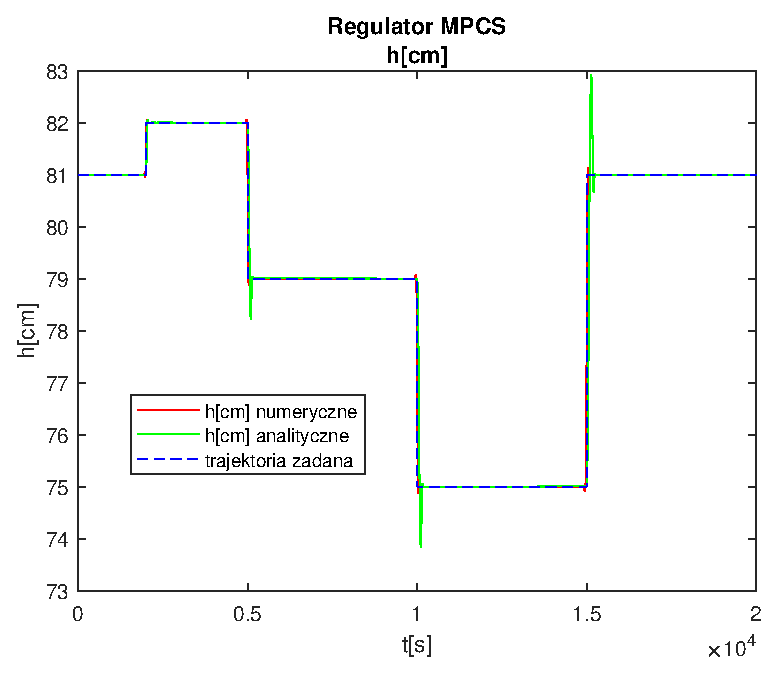
\includegraphics[width=1\linewidth]{img/MPCSnumRK/MPCSRKHN100Nu50l50.eps}
      \caption{}
      \label{fig:fig:MPCSRKN100Nu50l501}
   \end{subfigure}
       
   \begin{subfigure}[b]{0.4\textwidth}
      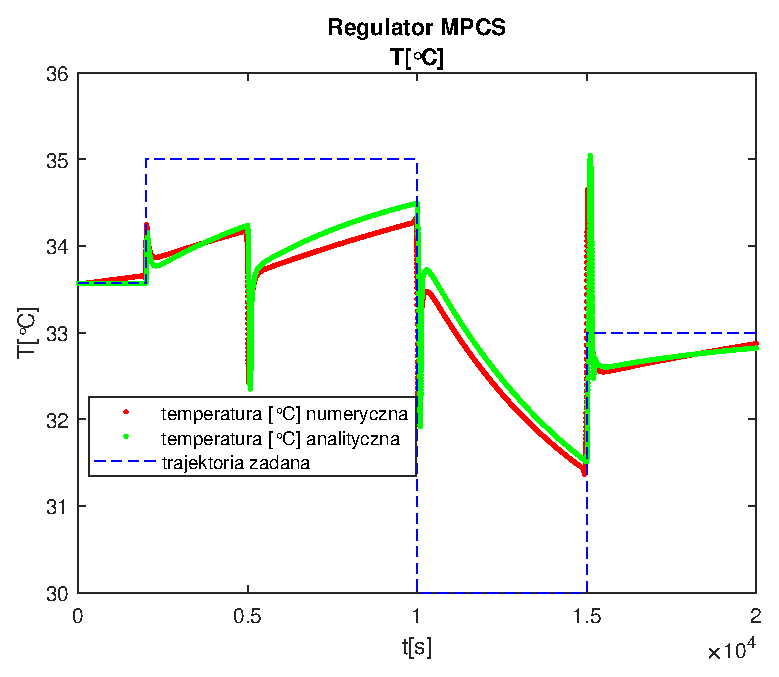
\includegraphics[width=1\linewidth]{img/MPCSnumRK/MPCSRKTN100Nu50l50.eps}
      \caption{}
      \label{fig:fig:MPCSRKN100Nu50l502}
   \end{subfigure}
       
   \begin{subfigure}[b]{0.4\textwidth}
      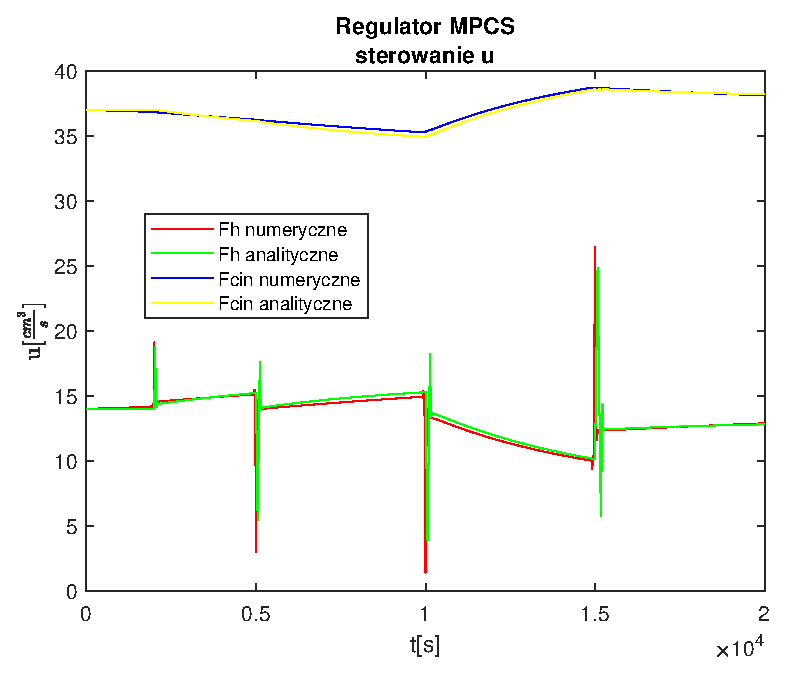
\includegraphics[width=1\linewidth]{img/MPCSnumRK/MPCSRKControlN100Nu50l50.eps}
      \caption{}
      \label{fig:fig:MPCSRKN100Nu50l503}
   \end{subfigure}
       
   \caption{Wykresy dla regulatora MPCS, obiekt nieliniowy, $N = 100$, $N_u = 50$.}
   \label{fig:MPCSRKN100Nu50l50}
\end{figure}
           

\FloatBarrier

\FloatBarrier
    \begin{figure}[h!]
   \centering
   \begin{subfigure}[b]{0.4\textwidth}
      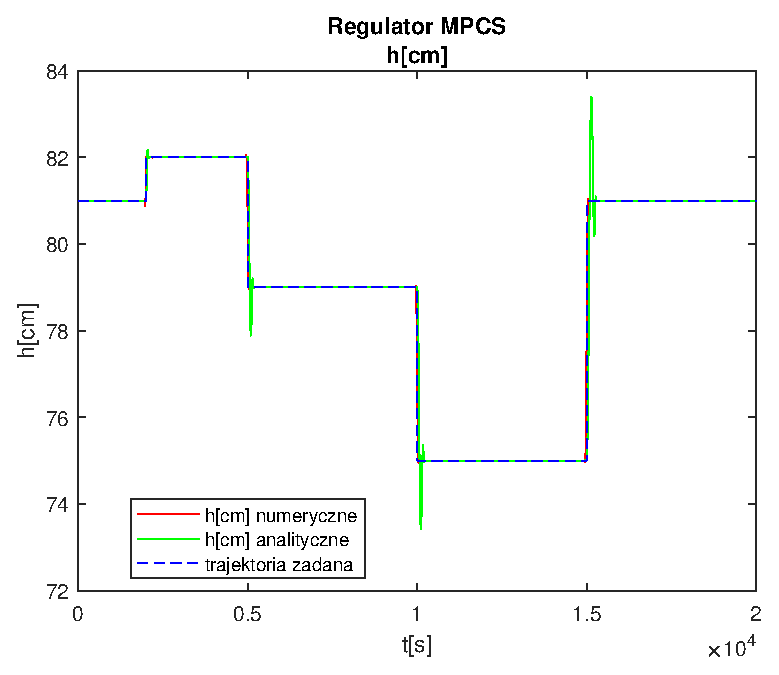
\includegraphics[width=1\linewidth]{img/MPCSnumRK/MPCSRKHN50Nu10l20.eps}
      \caption{}
      \label{fig:fig:MPCSRKN50Nu10l201}
   \end{subfigure}
       
   \begin{subfigure}[b]{0.4\textwidth}
      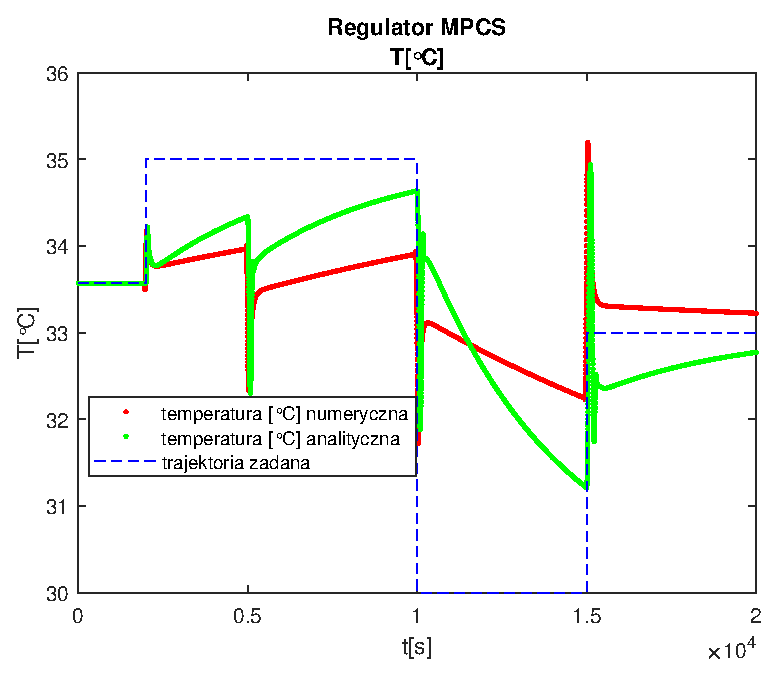
\includegraphics[width=1\linewidth]{img/MPCSnumRK/MPCSRKTN50Nu10l20.eps}
      \caption{}
      \label{fig:fig:MPCSRKN50Nu10l202}
   \end{subfigure}
       
   \begin{subfigure}[b]{0.4\textwidth}
      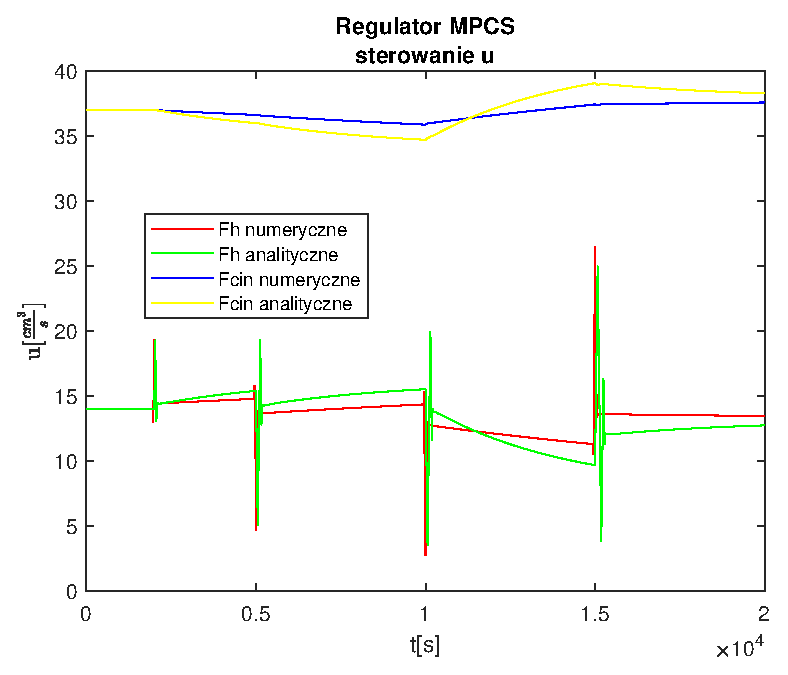
\includegraphics[width=1\linewidth]{img/MPCSnumRK/MPCSRKControlN50Nu10l20.eps}
      \caption{}
      \label{fig:fig:MPCSRKN50Nu10l203}
   \end{subfigure}
       
   \caption{Wykresy dla regulatora MPCS, obiekt nieliniowy, $N = 50$, $N_u = 10$, $\lambda = 0.2$.}
   \label{fig:MPCSRKN50Nu10l20}
\end{figure}
           

\FloatBarrier

\FloatBarrier
    \begin{figure}[h!]
   \centering
   \begin{subfigure}[b]{0.4\textwidth}
      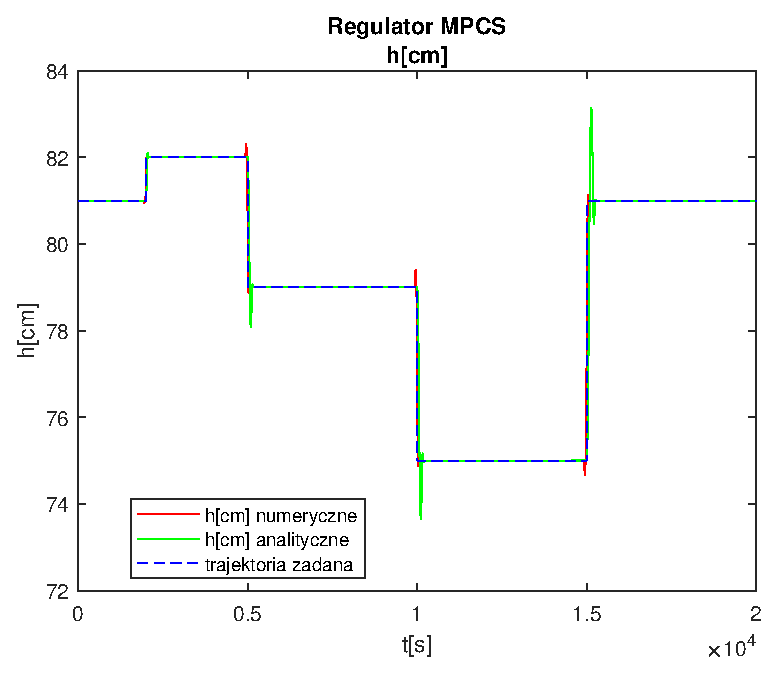
\includegraphics[width=1\linewidth]{img/MPCSnumRK/MPCSRKHN80Nu30l30.eps}
      \caption{}
      \label{fig:fig:MPCSRKN80Nu30l301}
   \end{subfigure}
       
   \begin{subfigure}[b]{0.4\textwidth}
      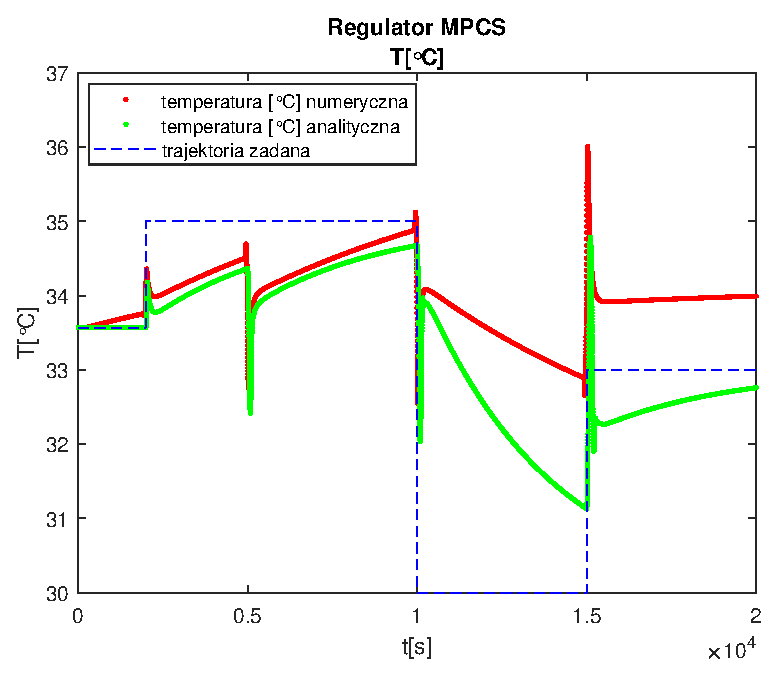
\includegraphics[width=1\linewidth]{img/MPCSnumRK/MPCSRKTN80Nu30l30.eps}
      \caption{}
      \label{fig:fig:MPCSRKN80Nu30l302}
   \end{subfigure}
       
   \begin{subfigure}[b]{0.4\textwidth}
      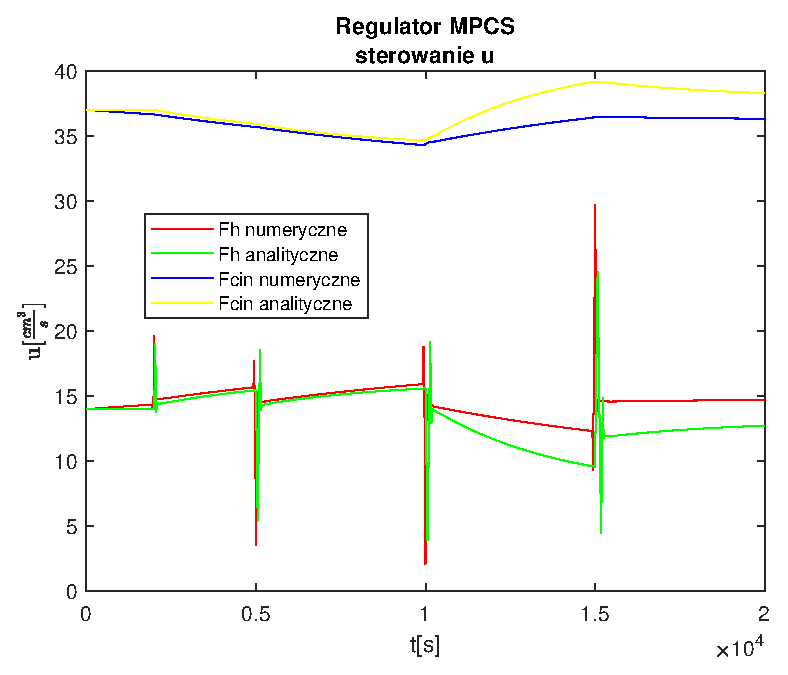
\includegraphics[width=1\linewidth]{img/MPCSnumRK/MPCSRKControlN80Nu30l30.eps}
      \caption{}
      \label{fig:fig:MPCSRKN80Nu30l303}
   \end{subfigure}
       
   \caption{Wykresy dla regulatora MPCS, obiekt nieliniowy, $N = 80$, $N_u = 30$, $\lambda = 0.3$.}
   \label{fig:MPCSRKN80Nu30l30}
\end{figure}
           

\FloatBarrier